\begin{frame}{Comparons nos intérêts}
  Avec un.e partenaire, discutez de vos intérêts en faisant des comparaisons.
  Utilisez des \emph{pronoms possessifs} autant que possible.
  \begin{columns}
    \column{0.6\textwidth}
      \only<1>{
        \begin{itemize}
          \small
          \item[] \textbf{Modèle:}
          \item[E1:] Ma musique préférée est la country.
          \item[E2:] \alert{La mienne} est la musique classique. Pourquoi est-ce que tu préfère la country?
        \end{itemize}
        \begin{center}
          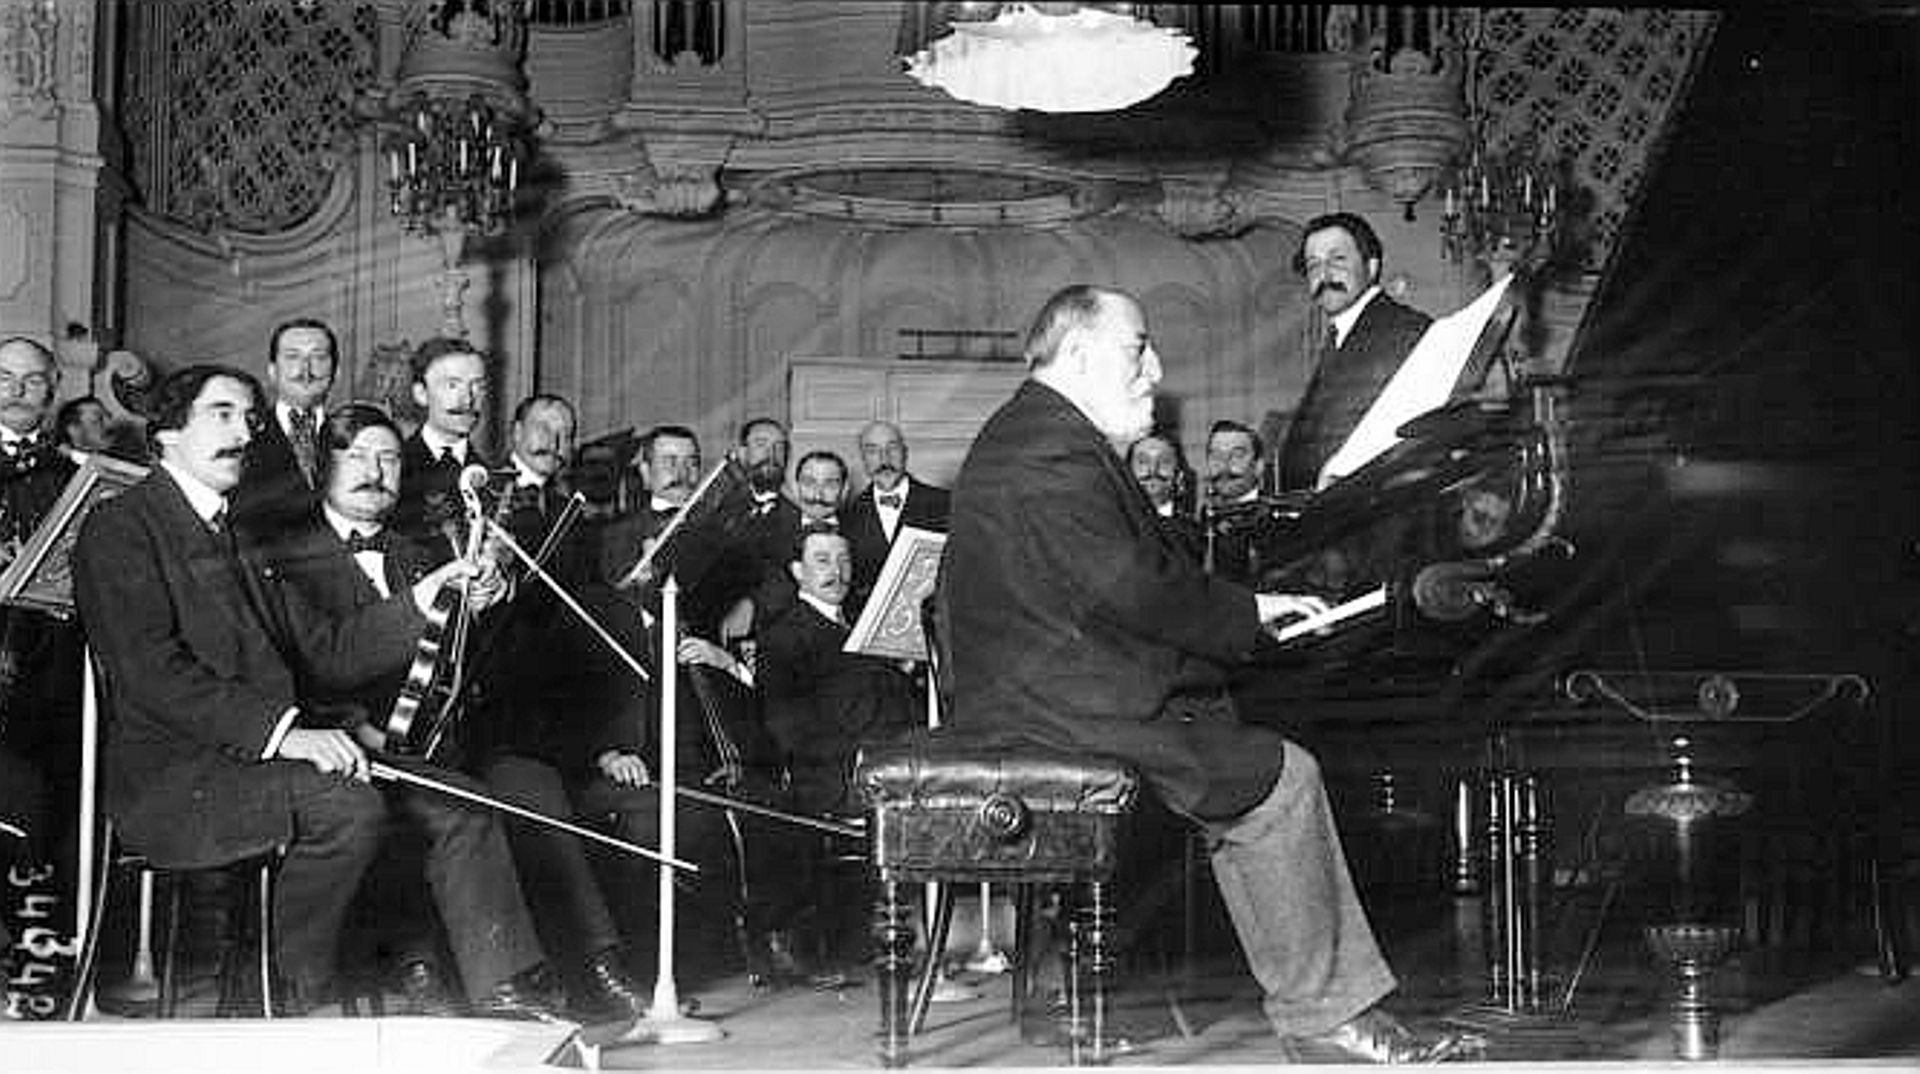
\includegraphics[scale=0.07]{saint-saens.jpg} \\
          {\scriptsize Camille Saint-Saëns en 1913}
        \end{center}
      }
      \only<2->{

        \vspace{0.25cm}
        \small
        Écrivez ce que vous et votre partenaire n'avez pas en commun.
        Utilisez le modèle suivant:
        \begin{itemize}
          \item Pour ce qui concerne nos <sujet> préféré.e.s, <pronom possessif> (mine) est/sont \underline{\hspace{2cm}} parce que \underline{\hspace{2cm}}, et <pronom possessif> (his/hers) est/sont \underline{\hspace{2cm}} parce que \underline{\hspace{2cm}}.
        \end{itemize}
      }
    \column{0.4\textwidth}
      \begin{minipage}[c][0.7\textheight]{\linewidth}
        Des sujets possibles:
        \begin{enumerate}
          \item La musique
          \item Les cours
          \item La nourriture
          \item Les films
          \item Les sports
          \item Les activités en plein air
          \item Le théâtre
          \item etc.
        \end{enumerate}
      \end{minipage}
  \end{columns}
\end{frame}